\section{Introduction}
\label{sec:intro}

LLM-as-a-judge has become a standard way to evaluate language models. Judges
rank systems on public leaderboards, supply the preference labels that train
reward models, and monitor other models' actions for safety. The judge and the
models it grades usually come from the same handful of systems, and judges are
known to rate their own outputs above others'
\citep{panickssery2024selfpreference, wataoka2024perplexity, ye2025justice}.
The standard defence is anonymisation: hide which model wrote each answer.
That defence holds only if a judge cannot tell from the text itself which
answers are its own, a capability known as \emph{self-recognition}.

Whether judges can recognise themselves matters in both directions. If they
can, anonymisation fails silently: a leaderboard can drift towards the judge's
own model, a reward model can learn the judge's style rather than quality, and
a monitor checking a copy of itself is no longer independent
\citep{khullar2026selfattribution}. If they cannot, then the self-preference
that judges show must come from somewhere else, and defences built around
hiding authorship are aimed at the wrong target.

\begin{figure}[t]
\centering
\begin{subfigure}[b]{0.49\linewidth}\centering
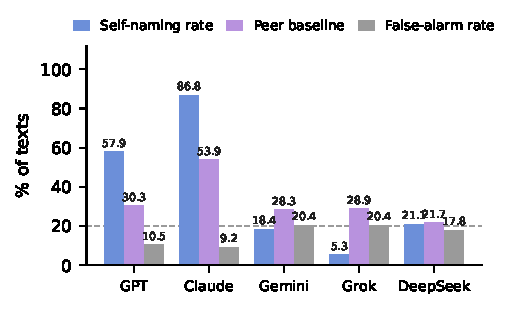
\includegraphics[width=\linewidth]{figures/lead_lineup.pdf}
\caption{Lineup of five answers}\label{fig:lead-lineup}
\end{subfigure}\hfill
\begin{subfigure}[b]{0.49\linewidth}\centering
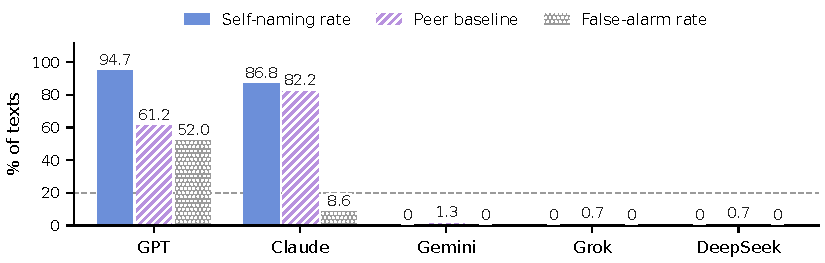
\includegraphics[width=\linewidth]{figures/lead_single.pdf}
\caption{One text at a time}\label{fig:lead-single}
\end{subfigure}
\caption{Figure~\ref{fig:lead-lineup} shows, for five frontier judges and 38
chat-app essays each, how often a judge names itself on its own essays
(self-naming rate), how often the other judges name it on those essays (peer
baseline), and how often it names itself on essays it did not write
(false-alarm rate). Claude and GPT beat their peers by 33 and 28 points; Grok
trails its peers. Figure~\ref{fig:lead-single} shows the same essays judged one
at a time: three judges never name themselves, GPT names itself on half of the
essays it did not write, and Claude's peers name Claude almost as often as
Claude does. The dashed line is the 20\% chance level.}
\label{fig:lead}
\end{figure}

Self-recognition is usually measured with one number: how often a judge names
itself as the author of its own text, compared with chance. We call this the
\emph{self-naming rate}, and we argue that it cannot answer the question on
its own. A judge that names itself on 87\% of its own answers may recognise
its writing. But the text may also be easy for \emph{any} model to attribute,
or the judge may simply say ``me'' to everything. The first case is a real
leak; the other two are not. Two further numbers from the same experiment tell
them apart: the \emph{false-alarm rate}, how often the judge names itself on
text it did not write, and the \emph{peer baseline}, how often the other judges
name it on its text (Figure~\ref{fig:lead}).

Prior evidence on self-recognition is contradictory.
\citet{panickssery2024selfpreference} report that models can recognise their
own outputs and link this to self-preference, while
\citet{davidson2024anonymized} find no consistent self-recognition in
anonymised panels, and \citet{bai2025selfrecognition} find accuracy near chance
when ten models are shown one text at a time. \citet{barkhordar2026stylenotself}
show for code that attribution accuracy mostly reflects how readily a model
claims authorship. These studies differ in models, texts and question formats,
and none compares a judge with how often \emph{other} judges attribute the same
text to it, so their conclusions are hard to reconcile.

To address this, we conduct a cross-evaluation study in which every model
serves as both author and judge. We evaluate nine judges, five frontier models
and four open-weight models, on three sets of texts: 190 essays the frontier
models wrote in their chat apps, 600 texts they wrote through the API in four
genres, and 480 texts the open-weight models wrote for the same 120 prompts.
Judges attribute the texts in three formats: a \emph{lineup} of answers to the
same prompt, \emph{one text at a time}, and the direct question ``Did you write
this text?''. In total we collect more than 19,000 authorship judgments.

Our findings reveal that most apparent self-recognition does not survive a peer
baseline. The usual test finds self-recognition in \SVPStd{} of \SVPCells{}
combinations of judge, text set and format; only \SVPProper{} pass our test,
which requires a judge both to beat its peers and to name itself more on its own
text than on others'. The cases that survive are large: in the lineup, Claude's
self-advantage over its peers is \ClaudeAdvLineup{} points \ClaudeAdvLineupCI{}
and GPT's is \GPTAdvLineup{} \GPTAdvLineupCI{}. Yet on 600 API texts from the same models no
judge beats its peers. The format alone reshapes the results. One text at a
time, judges send \SingleConcentration{} of all guesses to GPT or Claude, and
asked directly, GPT, Grok and DeepSeek deny writing any of the 190 essays,
their own included, a pattern we call \emph{self-denial}. Open-weight judges
show the opposite, \emph{over-attribution}: Llama names itself on every text it
is shown one at a time.

To understand these failures, we test what the judges rely on. The signal they
would need is present: a classifier over 18 style features attributes
\EngineAAcc{} of the essays, and each open-weight judge finds its own text the
most likely one on every prompt. Yet the judges' answers follow neither their
own likelihoods, nor the similarity of a text to their own writing, nor its
quality. With each essay's words shuffled, a bag-of-words classifier still
attributes \BowShufAcc{} while the judges fall to chance. Their stated reasons
reveal stereotypes of each model that they apply to every text alike.

In summary, we show that the standard test of LLM self-recognition is
unreliable, and we provide a corrected test that needs no data beyond what a
lineup already collects. Self-recognition, where it exists, is a property of a
particular judge on particular texts in a particular format, not a fixed trait
of a model. Anonymised evaluation should therefore be audited per judge, on the
texts it will actually judge, against a peer baseline.
